% Le titre de la partie
\section{\cclpti}

%%%%%%%%%%%%%%%%%%%%%%%%%%%%%%%%%%%%%%%%%%%%%%%%
% Première diapo
%%%%%%%%%%%%%%%%%%%%%%%%%%%%%%%%%%%%%%%%%%%%%%%%
\begin{frame}
    \frametitle{\cclpti}
    \framesubtitle{}
    
    \centering {\huge \cclpti}
    
    \end{frame}

%%%%%%%%%%%%%%%%%%%%%%%%%%%%%%%%%%%%%%%%%%%%%%%%
% Deuxième diapo
%%%%%%%%%%%%%%%%%%%%%%%%%%%%%%%%%%%%%%%%%%%%%%%%
\begin{frame}
    \frametitle{\cclpti}
    \framesubtitle{La simulation}
    
    \centering
    \onslide*<1>{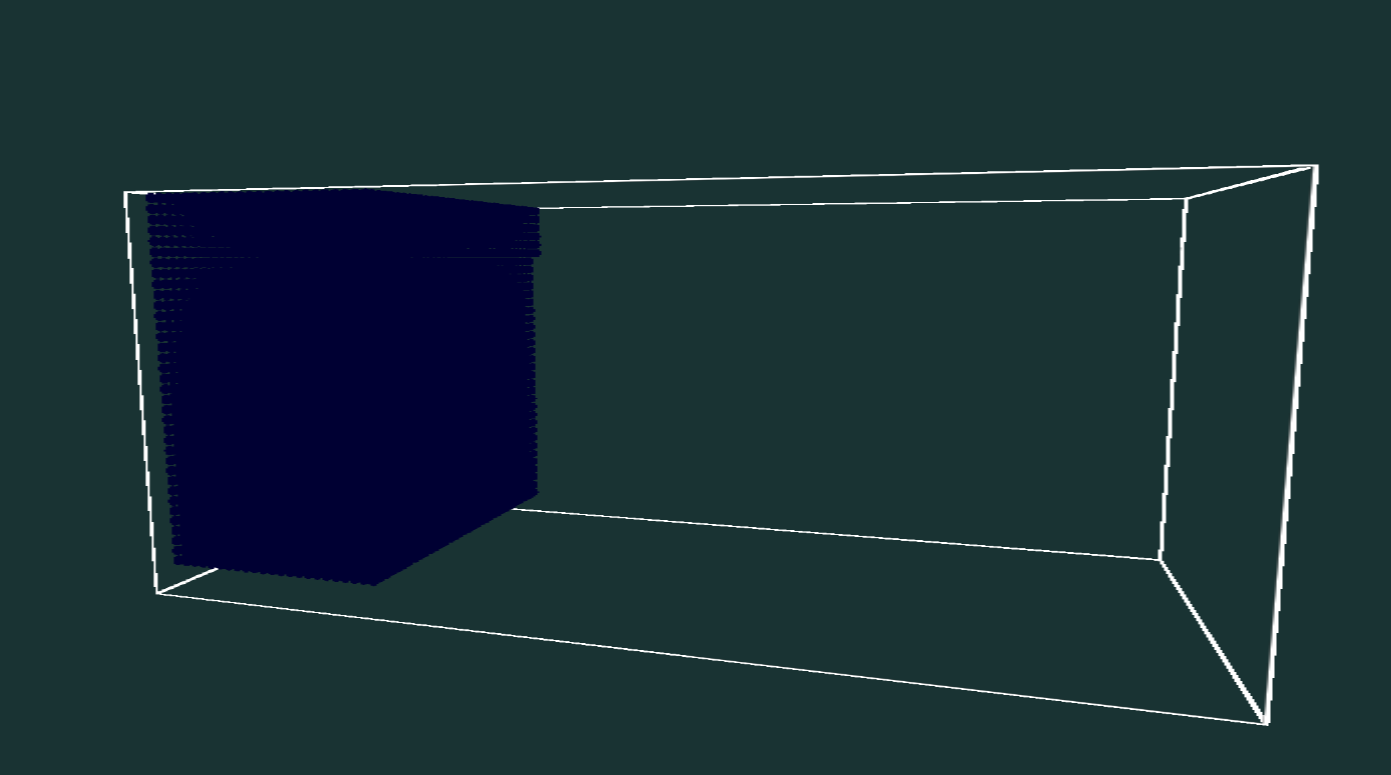
\includegraphics[width=1.0\linewidth]{figures/fluid_sim_finale_1.png}}
    \onslide*<2>{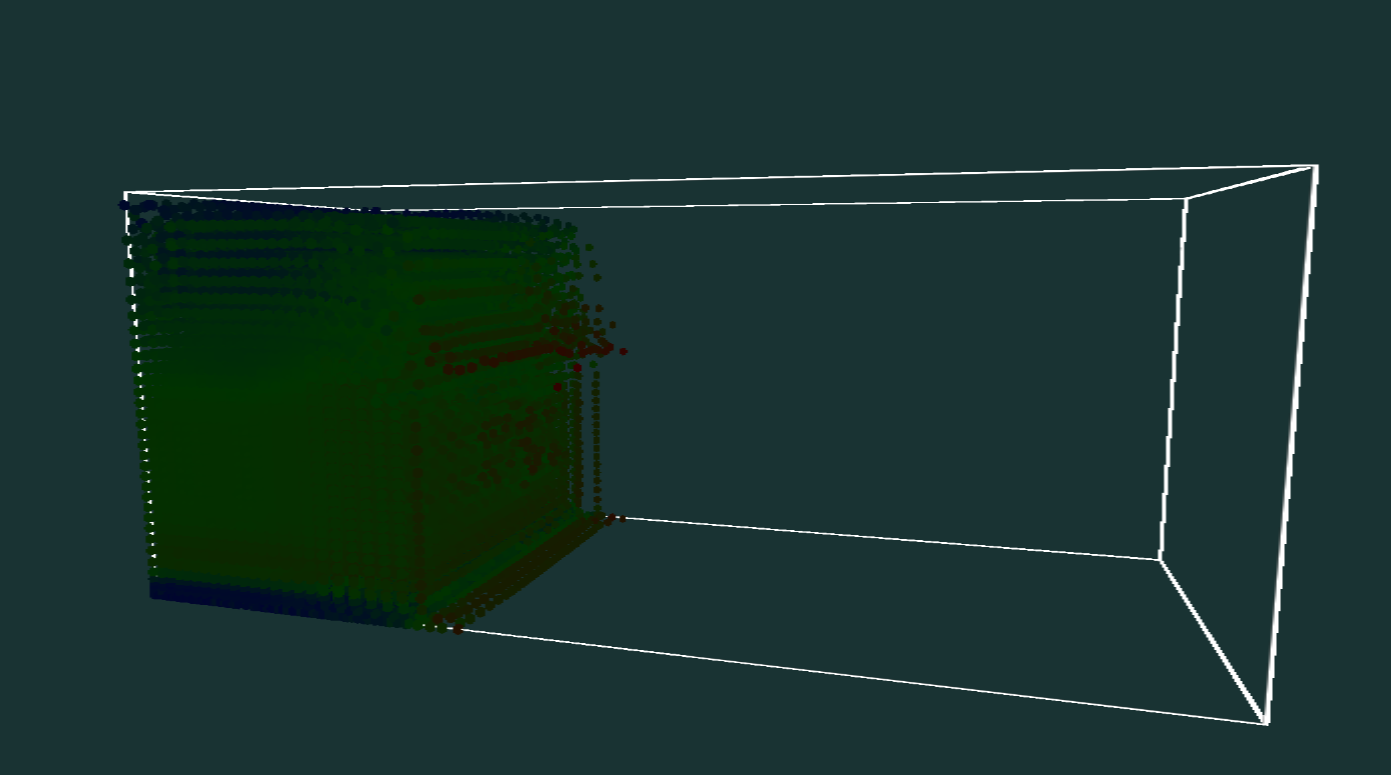
\includegraphics[width=1.0\linewidth]{figures/fluid_sim_finale_2.png}}
    \onslide*<3>{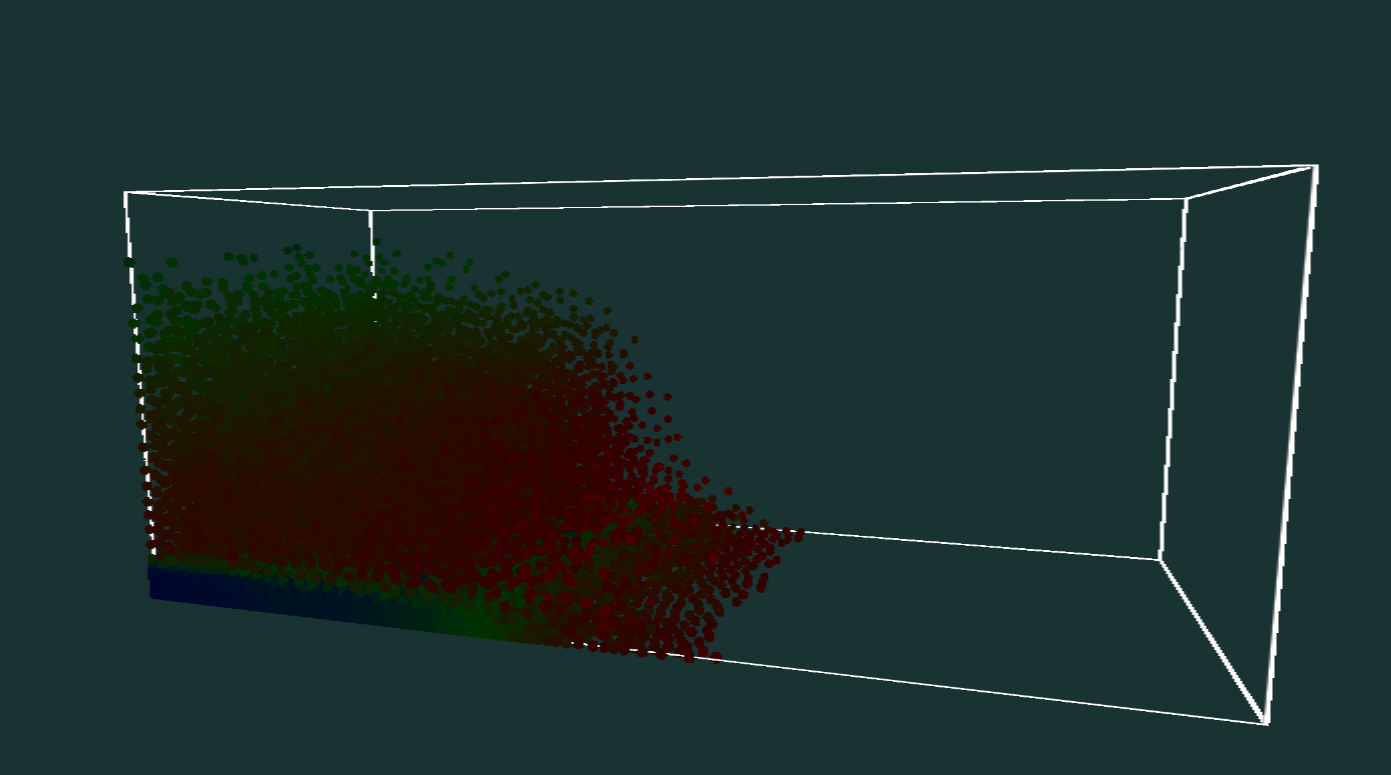
\includegraphics[width=1.0\linewidth]{figures/fluid_sim_finale_3.png}}
    \onslide*<4>{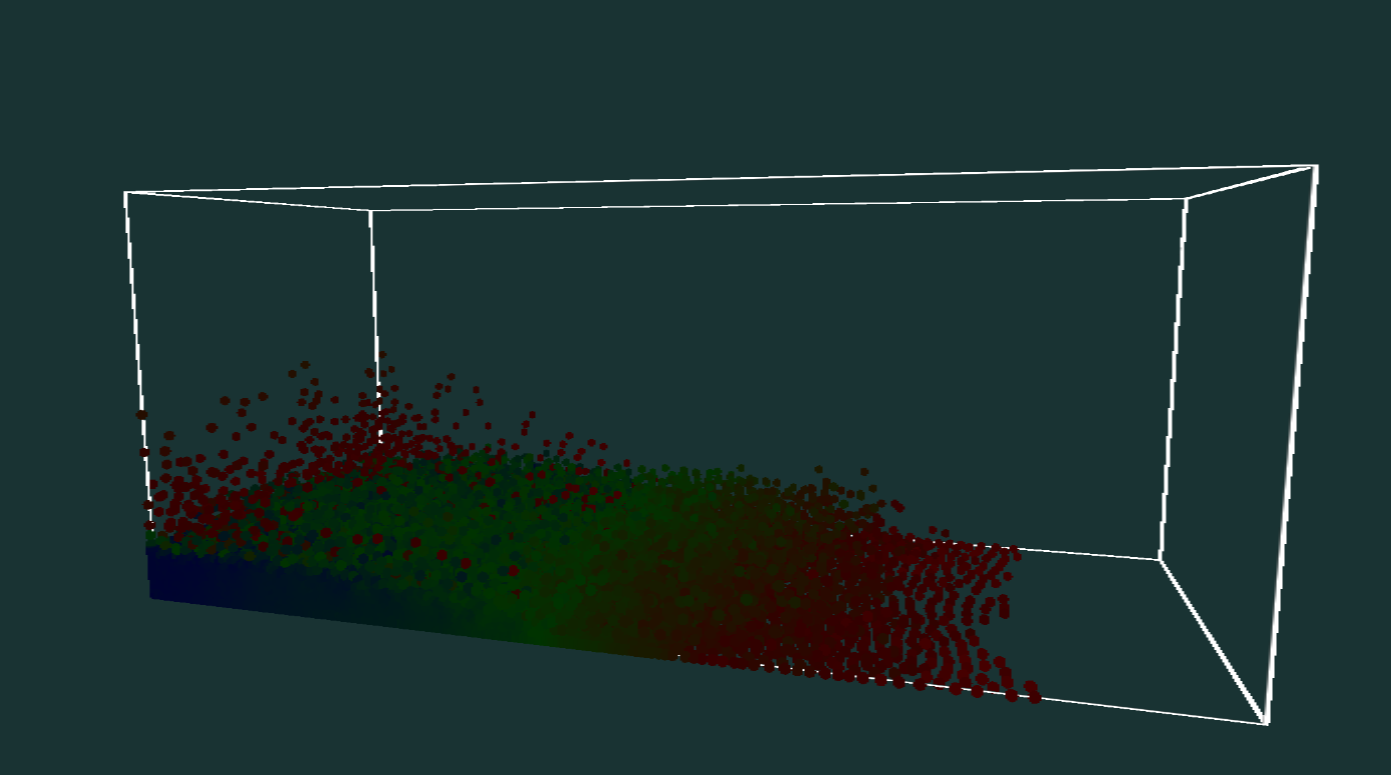
\includegraphics[width=1.0\linewidth]{figures/fluid_sim_finale_4.png}}
    \onslide*<5>{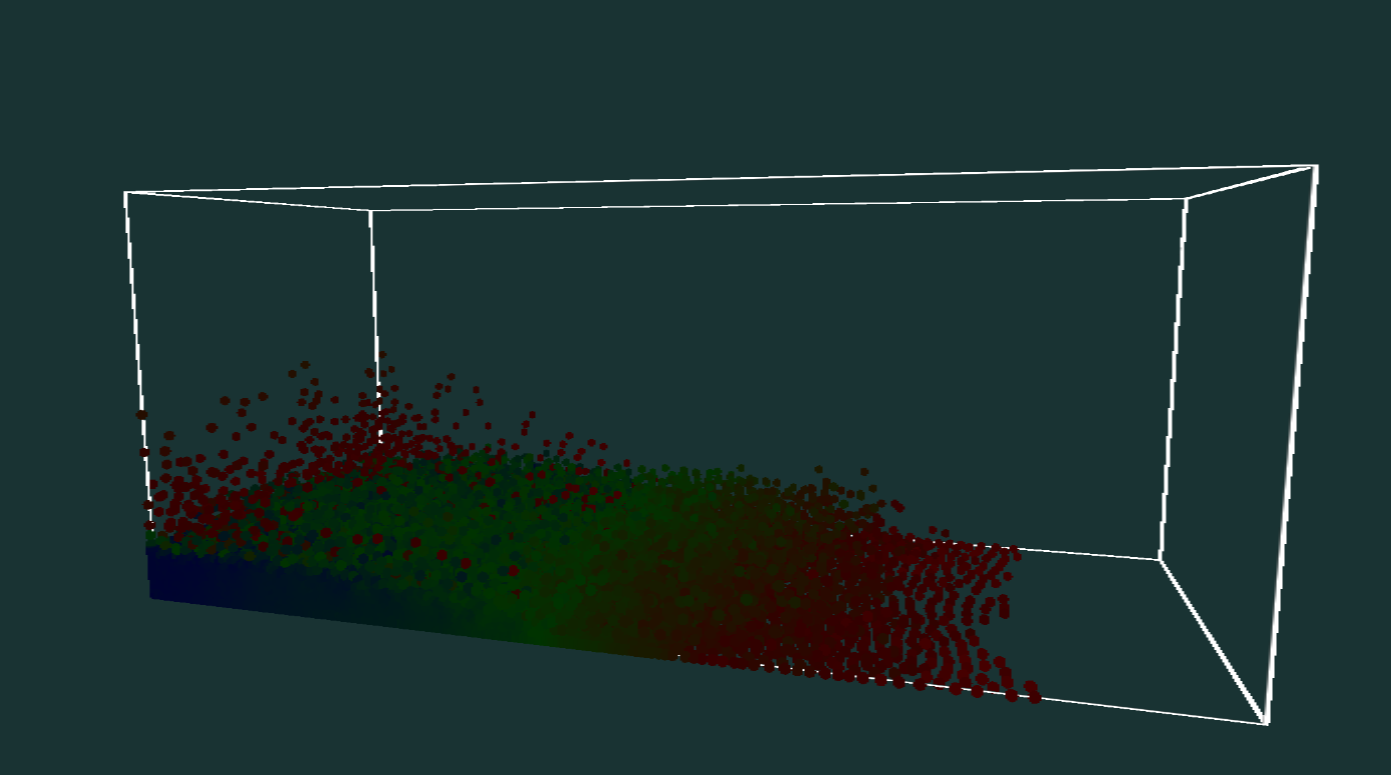
\includegraphics[width=1.0\linewidth]{figures/fluid_sim_finale_5.png}}
    \onslide*<6>{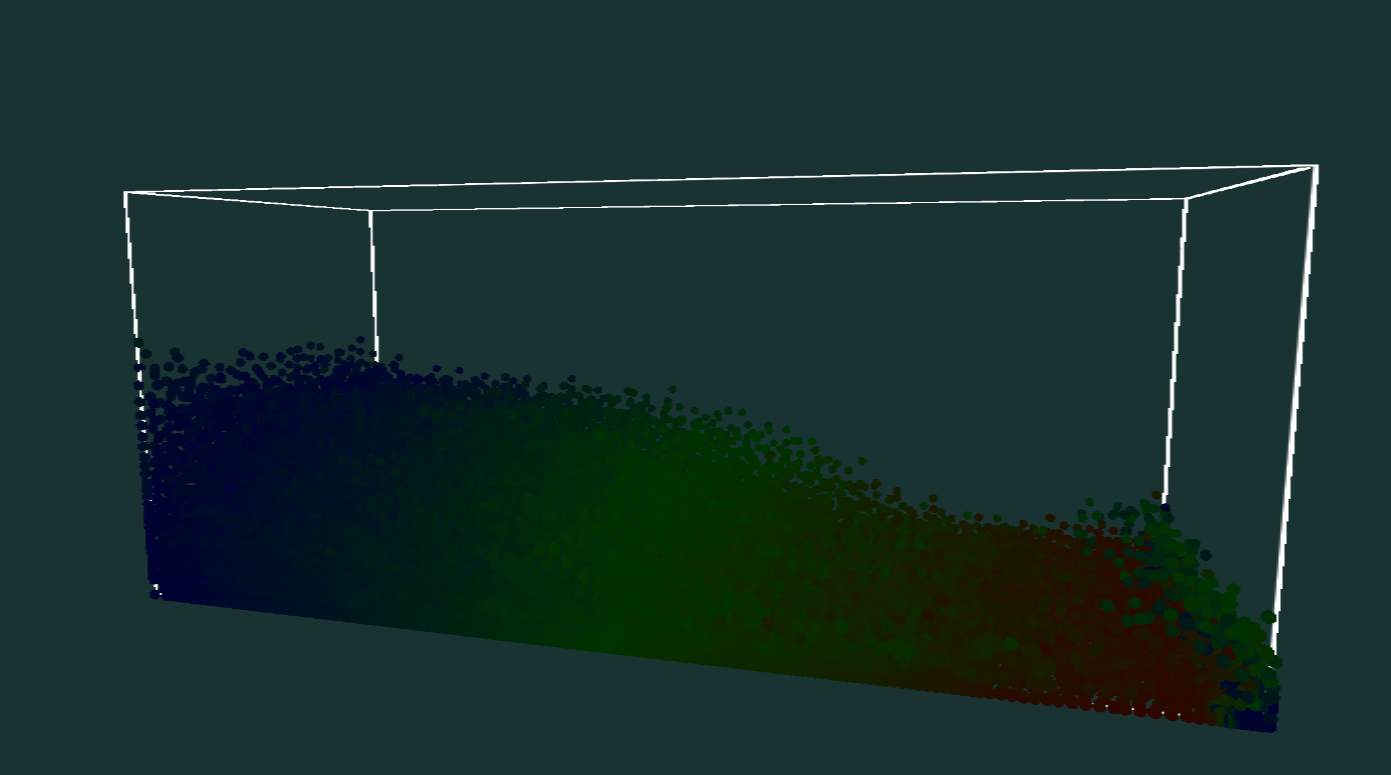
\includegraphics[width=1.0\linewidth]{figures/fluid_sim_finale_6.png}}
    \onslide*<7>{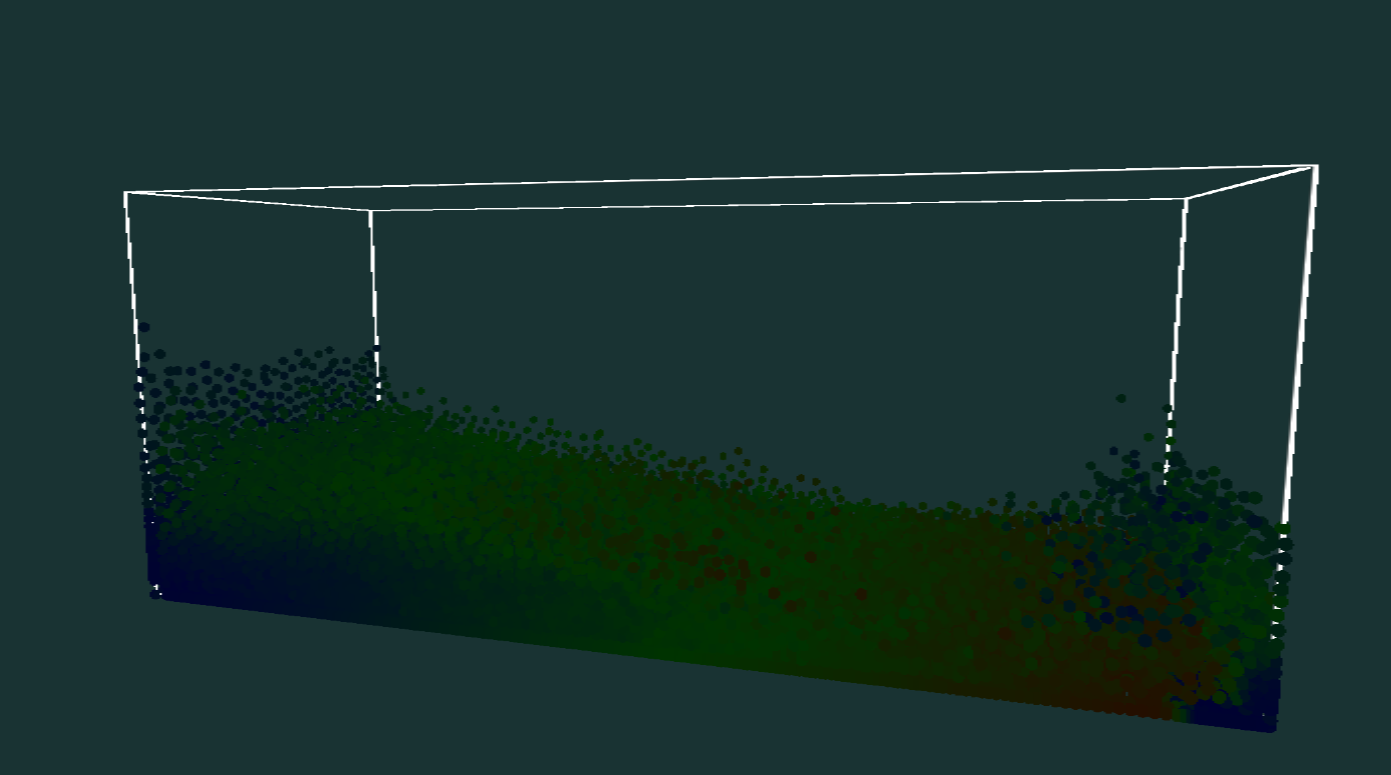
\includegraphics[width=1.0\linewidth]{figures/fluid_sim_finale_7.png}}
    \onslide*<8>{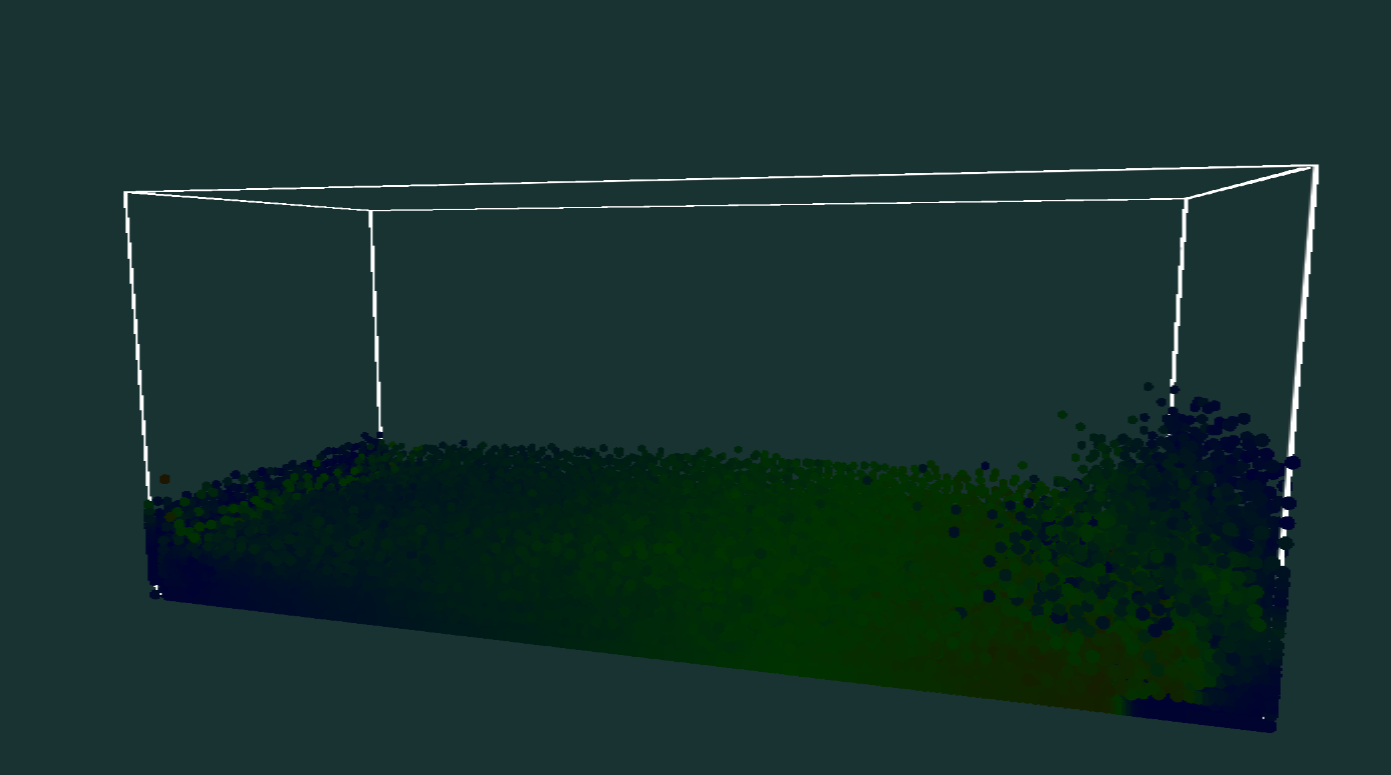
\includegraphics[width=1.0\linewidth]{figures/fluid_sim_finale_8.png}}
    \onslide*<9>{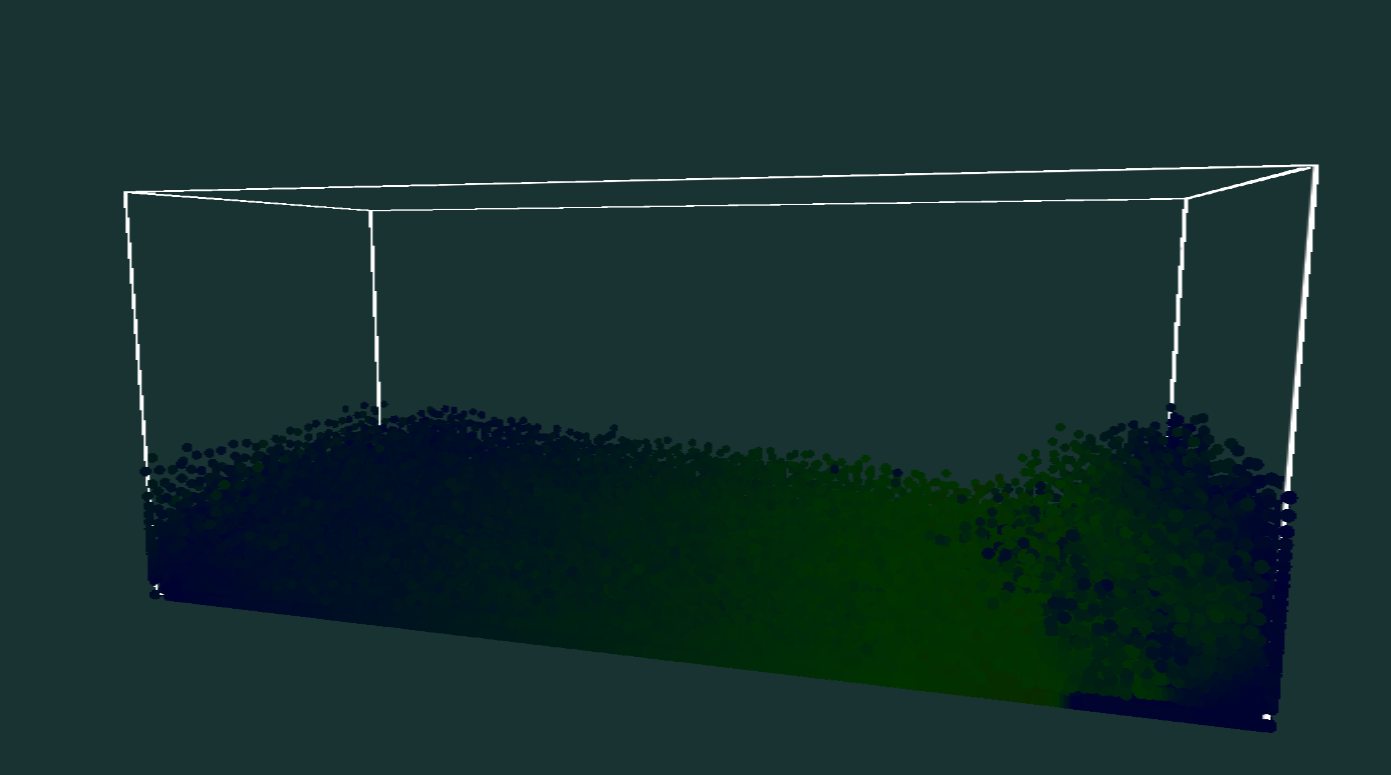
\includegraphics[width=1.0\linewidth]{figures/fluid_sim_finale_9.png}}
    \onslide*<10>{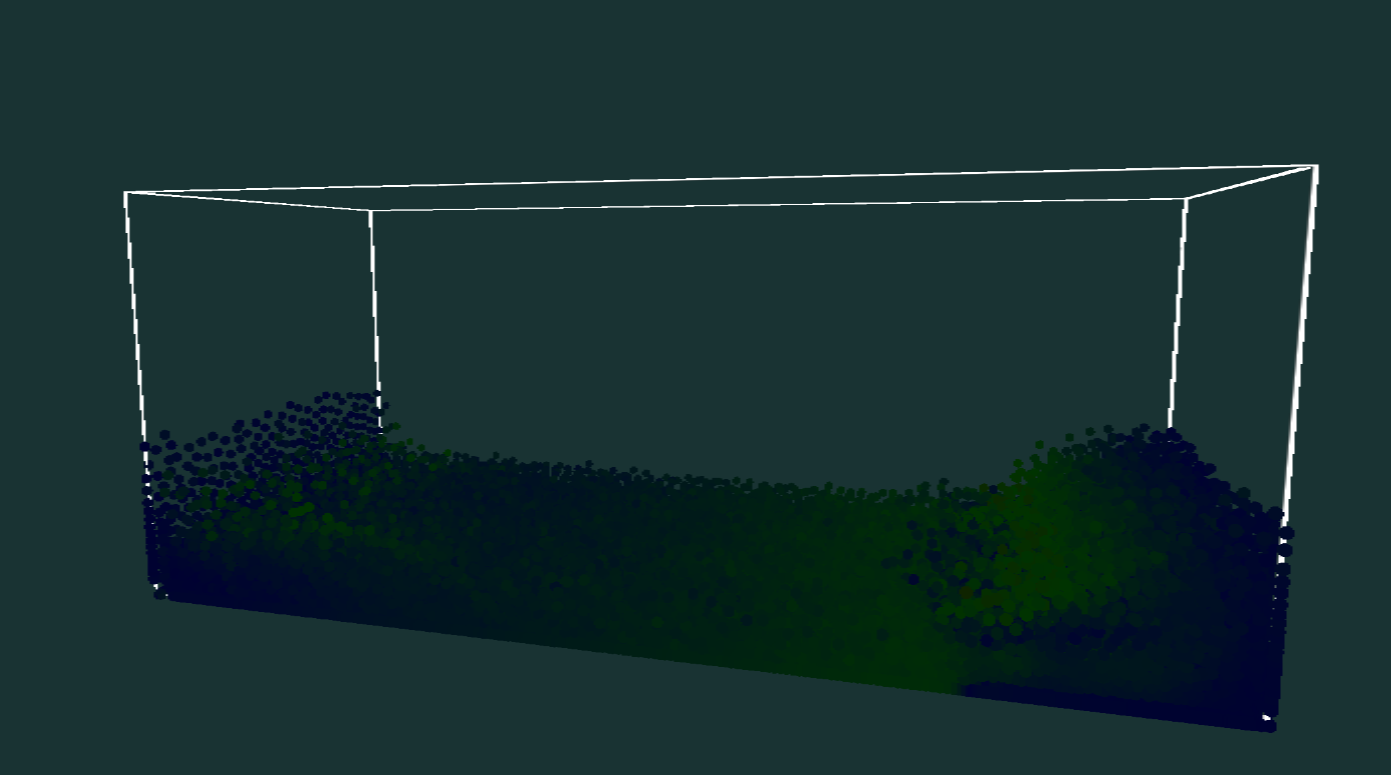
\includegraphics[width=1.0\linewidth]{figures/fluid_sim_finale_10.png}}
    \onslide*<11>{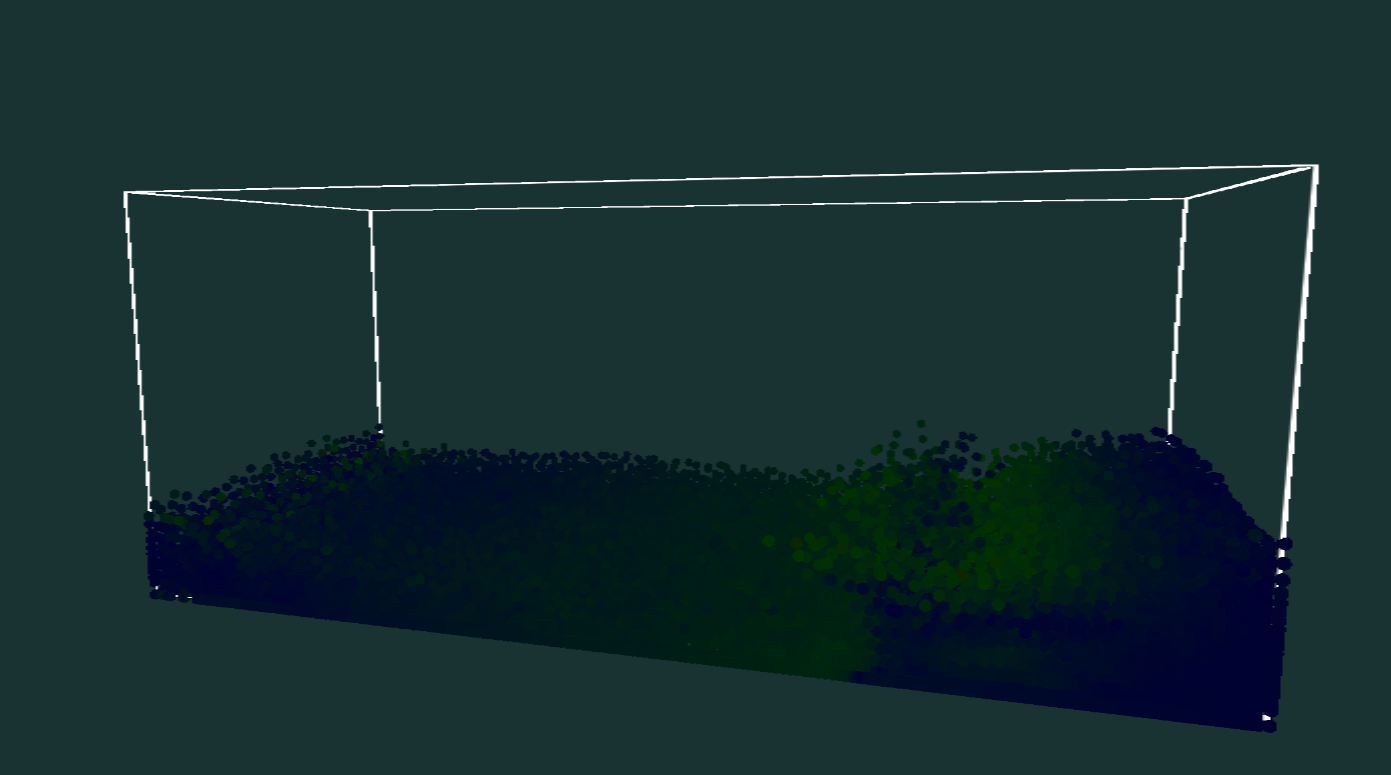
\includegraphics[width=1.0\linewidth]{figures/fluid_sim_finale_11.png}}
    \onslide*<12>{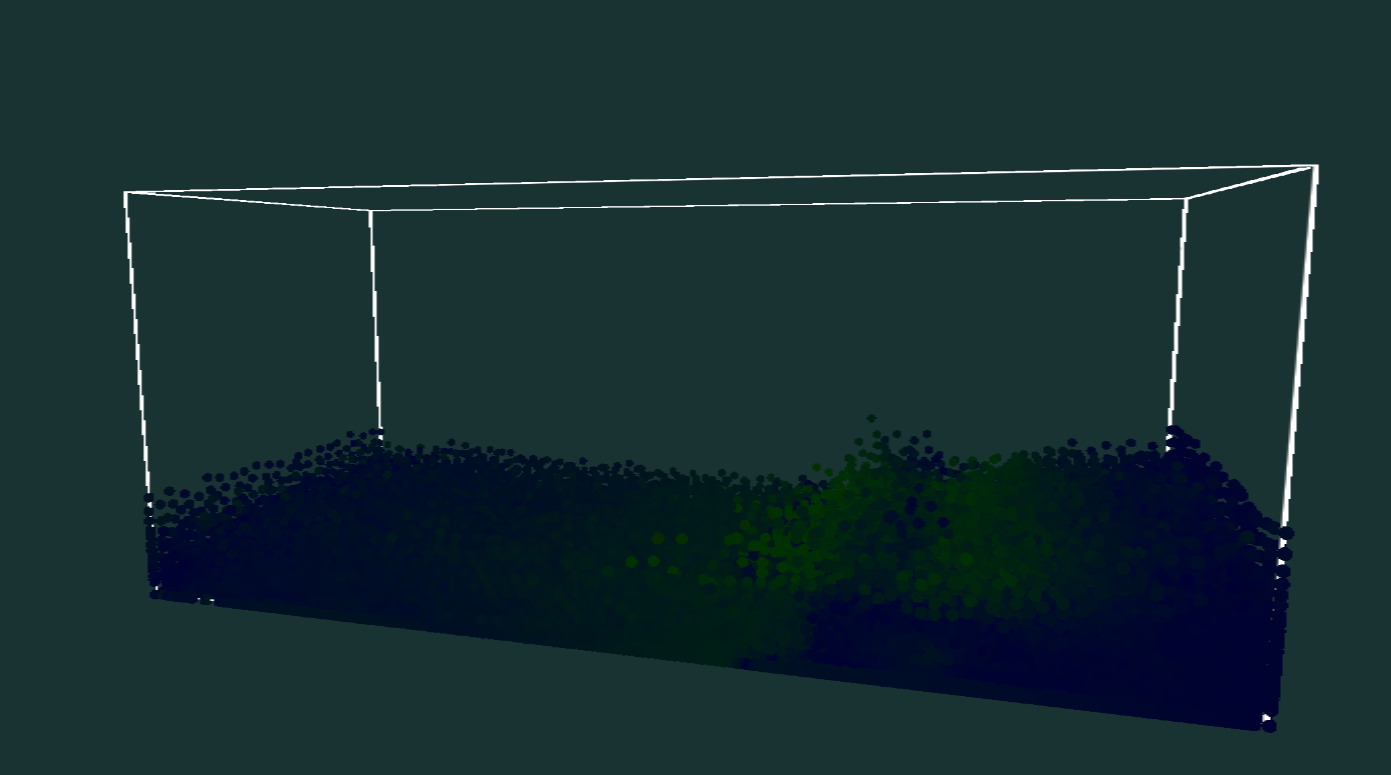
\includegraphics[width=1.0\linewidth]{figures/fluid_sim_finale_12.png}}
    \onslide*<13>{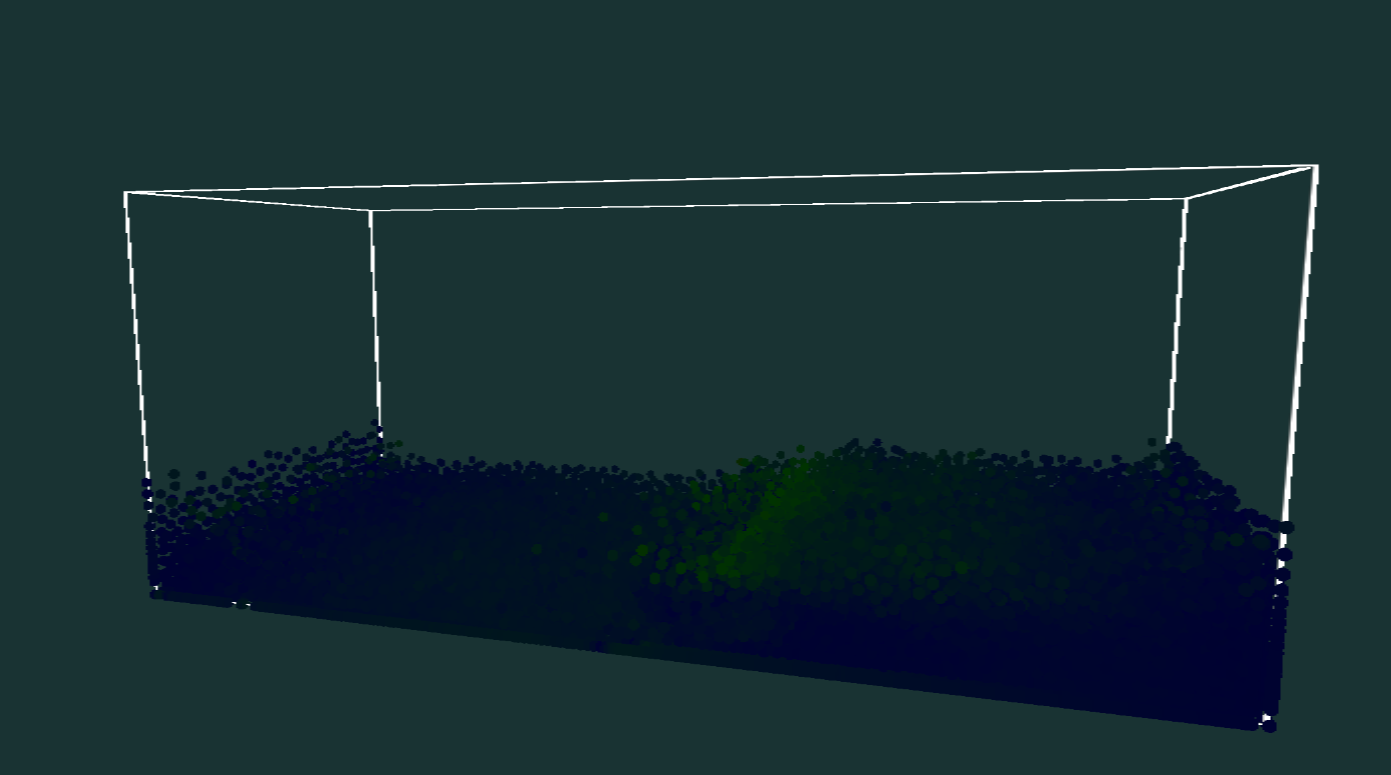
\includegraphics[width=1.0\linewidth]{figures/fluid_sim_finale_13.png}}
    \onslide*<14>{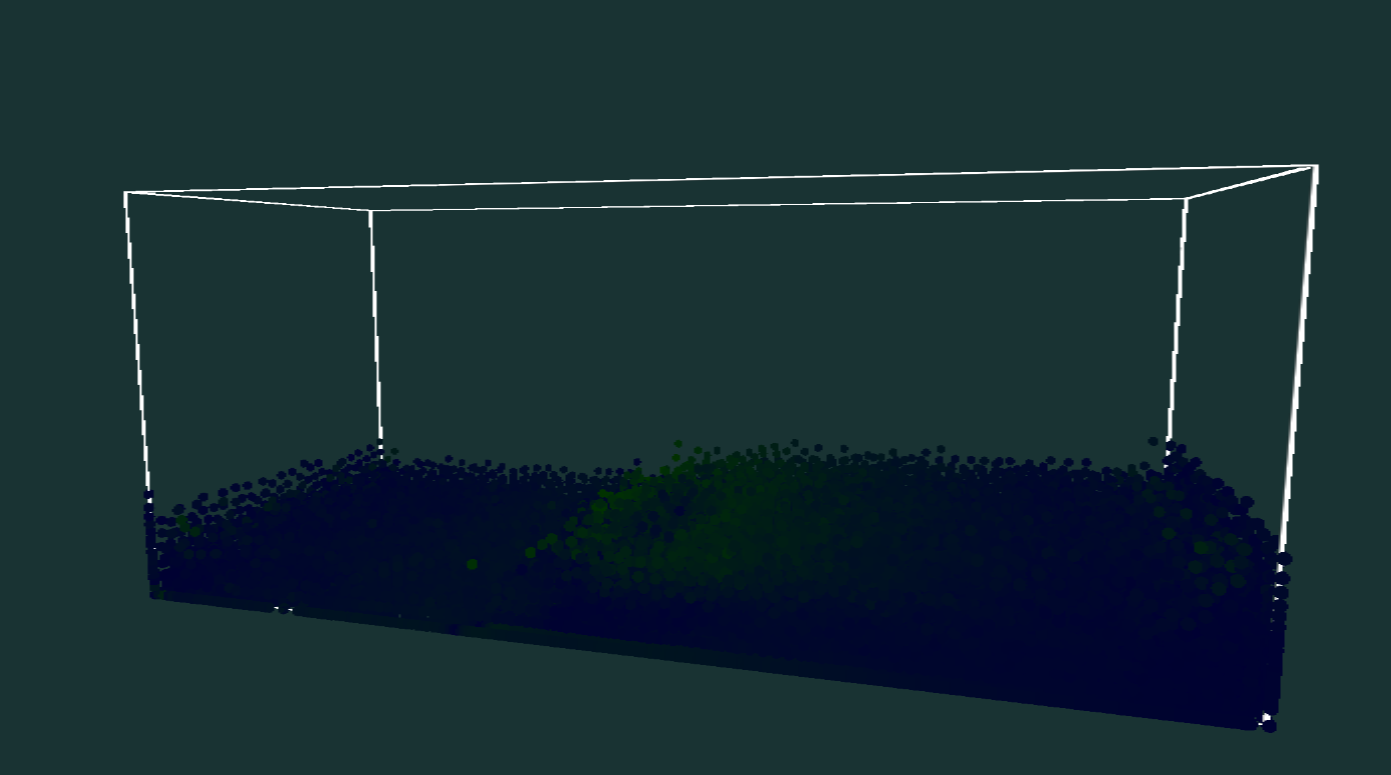
\includegraphics[width=1.0\linewidth]{figures/fluid_sim_finale_14.png}}
    \onslide*<15>{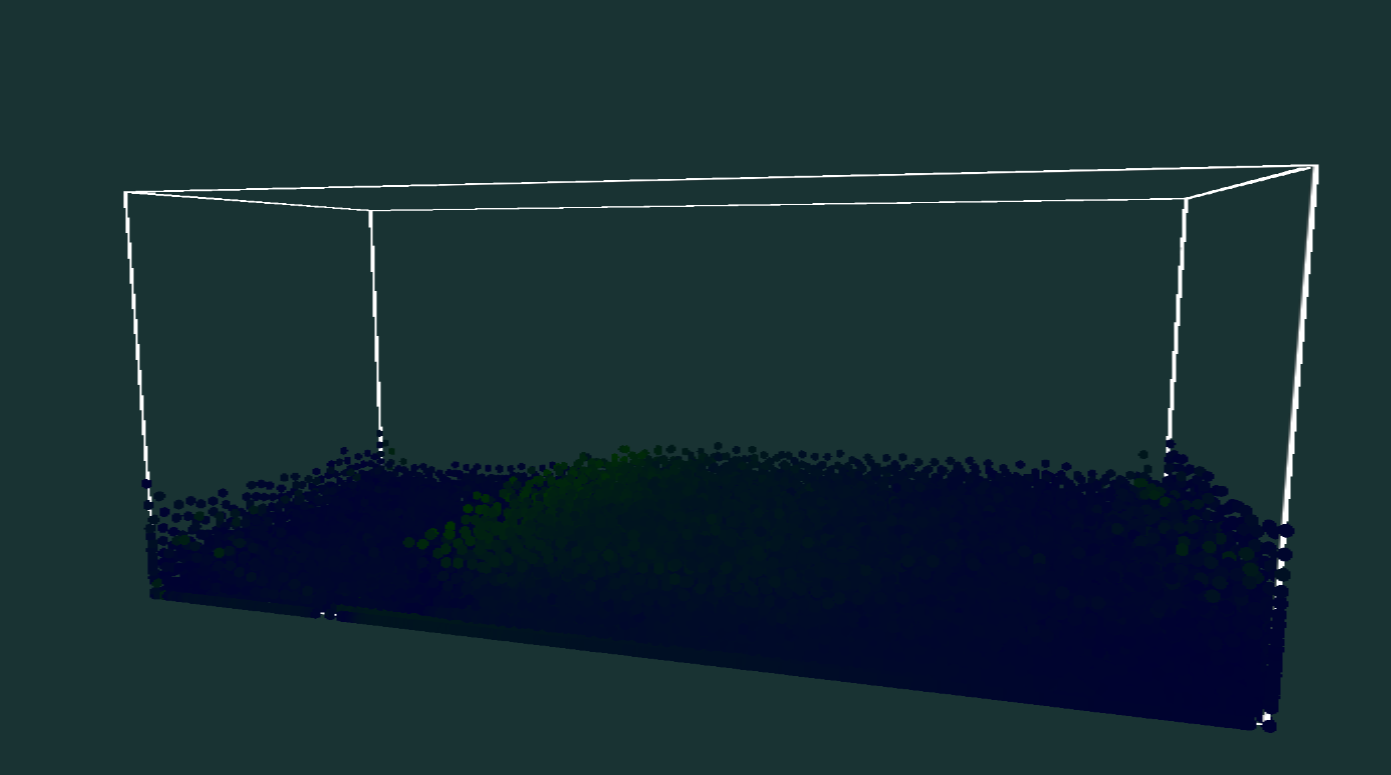
\includegraphics[width=1.0\linewidth]{figures/fluid_sim_finale_15.png}}

\end{frame}

%%%%%%%%%%%%%%%%%%%%%%%%%%%%%%%%%%%%%%%%%%%%%%%%
% 3eme diapo
%%%%%%%%%%%%%%%%%%%%%%%%%%%%%%%%%%%%%%%%%%%%%%%%
\begin{frame}
    \frametitle{\cclpti}
    \framesubtitle{Impact de l'optimisation}
    Nombre de particules maximum pour que la simulation tourne à 60 images par secondes:
    
    \begin{center}
        \begin{tabular}{ |c|c|c| } 
         \hline
         Ajout & Avant & Après \\ 
         \hline
         Passage sur la carte graphique & 350 & 5000 \\ 
         Ajout du partitionnement de l'espace & 5000 & 20.000 \\ 
         Ajout du tri bitonique & 20.000 & 60.000 \\
         \hline
        \end{tabular}
    \end{center}
    
    {\tiny Matériel:
    \begin{itemize}
        \item Processeur: Intel i7-6700 (8) @ 4.0GHz
        \item Carte Graphique: NVIDIA GeForce GTX 1060 6GB
        \item Mémoire Vive: 16Go
    \end{itemize}
    }
    \end{frame}
